%--------------------------------------------------------------------
%	(c) SPP 2014
%   This is a pragmatic LaTeX conversion of the MS Word document
%   stating the required format for the submission of articles 
%   for consideration in the SPP Physics Congress.  This template
%   includes the rules on formatting your article and thus before
%   editing it typeset it first to produce a postscript/pdf file
%   that you can read.  Use the latex, dvips, and ps2pdf commands 
%   to typeset the template directly into a pdf file.  Make sure 
%   to place the included figure in the same directory as the 
%   template.  This template uses standard LaTeX packages latexsym,
%   graphicx, geometry, fancyhdr, caption, and cite.
%
%   Note, in particular, the format used to typeset figures and
%   tables.  Since SPP requires figure/table captions to be
%   within an inch of the figure/table, you must define manually
%   the width of the caption at the beginning of the figure/table
%   environment.
%-------------------------------------------------------------------
\documentclass[twoside]{article}

\usepackage{latexsym}      % needed math symbols
\usepackage{graphicx}      % for importing eps figures

% paper and margin formats as set by SPP
\usepackage[margin=1.0in,papersize={21.0cm,29.7cm}]{geometry}

\parindent 0.5cm    % paragraphs indent
\newcommand{\changefont}{%
    \fontsize{9}{10}\selectfont
}

% for the footer
\usepackage{fancyhdr}
\fancyhf{}
\renewcommand{\headrulewidth}{0pt}
\renewcommand{\footrulewidth}{0.5pt}
\tiny
\fancyfoot[c]{\changefont
Physics 191 - Analysis and simulation of Lissajous curves \\
National Institute of Physics, Diliman, Quezon City\\
1 September 2016 \\
\thepage}

\pagestyle{fancy}

% for section formatting style
\makeatletter
\renewcommand\section{\@startsection
   {section}{1}{0pt}%
   {-\baselineskip}%
   {0.1\baselineskip}%
   {\normalfont\large\bfseries}}%
\makeatother
\renewcommand\thesection{\arabic{section}.}

% for the figure captions
\usepackage{caption}
\captionsetup[table]{position=top,aboveskip=5pt,font={rm,small}}
\captionsetup[figure]{font={rm,small}}

% for citations formatting style
\usepackage[compress,nospace]{cite}

\begin{document}

%--------------------------------------------------------------------------
%  fill in the paper's title, author(s), and corresponding institutions
%--------------------------------------------------------------------------
\begin{center}
{\Large\textbf{Analysis and simulation of Lissajous curves}}\\
\vspace{0.05in}
\textbf{Jan Carlo Lima$^1$, Marc Christian Perez$^1$, and Jhames Ni\~{n}o Trinidad$^{1 \ast}$}\\
\textit{$^1$National Institute of Physics, Diliman, Quezon City}\\
\textrm{$^{\ast}$Corresponding author: jtrinidad@nip.udp.edu.ph}\\

\vspace{0.15in}

%--------------------------------------------------------------------------
%                    write your abstract here
%--------------------------------------------------------------------------
\parbox{4.5in}{{\large \textbf{Abstract}}\\
\noindent{The experiment aims to simulate Lissajous patterns using an oscilloscope and two function generators and to explain their formation with their frequency ratio and phase difference. Patterns are observed in different frequency integer ratios where integers ranges from $1$ to $5$ with a phase difference equal to $0$, $\pi$, or $\frac{\pi}{2}$. It is found that these patterns can be derived by inputting values for amplitude, frequency, and phase difference into the simple harmonic motion equations of the two sinusoidal functions generated. }\\

\noindent{Keywords: Lissajous curve, frequency ratio, phase difference}}\\
\end{center}

%---------------------------------------------------------------------------
%               the main text of your paper begins here
%---------------------------------------------------------------------------
\section{Introduction}
\label{sec:intro}

The central limit theorem states that for a random variable $x$, the arithmetic mean of $n$ independent trials of $x$ will be approximately normally distributed if $n$ is a large number \cite{walpole}. The theorem relates the arithmetic mean $\bar{x}$ of a random variable $x$ given by Equation \ref{mean} to the normal (Gaussian) distribution given by Equation \ref{Gaussian}.

\begin{equation}
\bar{x} = \frac{1}{N}\sum_{i=1}^{\i=N}x_i
\label{mean}
\end{equation}

\begin{equation}
g(x)=Ae^{\frac{-(x-\bar{x})^2}{(2\sigma_x^2)}}
\label{Gaussian}
\end{equation}

The central limit theorem can be explained as follows: suppose a researcher has a distribution, not necessarily normal, but could look as weird as he wishes. Then, he takes the average of $N$ measurements that follow that distribution, and it is these that he plots in a histogram. If $N = 1$, the histogram’s shape will look more like the original distribution. However, if he increases $N$, the resulting histogram for that $N$ would approach a normal distribution, and would look steeper (i.e. a smaller standard deviation) and the value at the peak would correspond to the arithmetic mean of all the random variables \cite{khan}. For a large number of trials $n$ of the values obtained from averaging $N$ random variables for each trial, the distribution function approaches the shape of the Gaussian (normal) distribution function.

In this experiment, the central limit theorem is demonstrated using pieces of 12-faced dice. The statistical properties of the random variables were studied in terms of how the number of averages affects the shape of the probability distribution.

%-------------------------------------------------------------------------
%                              Section 2
%-------------------------------------------------------------------------
\section{Methodology}
\label{sec:metho}

Two function generators were connected to the horizontal(x) and vertical(y) input of an oscilloscope. Both produced sine waves and were observed in the xy-plot display of the oscilloscope. While amplitudes of x and y inputs remained equal to each other, different patterns were observed as their frequencies and phase difference were varied. In each pattern, both frequencies and their phase difference were recorded. The different frequencies for x and y are listed below. 

\captionsetup[table]{width=4in}
\begin{table}[h!]
\centering
\caption{Nine ratios were used for this experiment.}
\begin{tabular}{||c|c|c||}
\hline
Ratio of y to x (y:X) & $y$ (kHz) & $x$ (kHz) \\ \hline \hline
$1:1$ & $1.00$ & $1.00$ \\ \hline
$1:2$ & $1.00$ & $2.00$ \\ \hline
$1:3$ & $1.00$ & $3.00$ \\ \hline
$2:1$ & $1.00$ & $0.50$ \\ \hline
$3:1$ & $3.00$ & $1.00$ \\ \hline
$2:3$ & $2.00$ & $3.00$ \\ \hline
$3:2$ & $3.00$ & $0.10$ \\ \hline
$2:5$ & $2.00$ & $5.00$ \\ \hline
$5:2$ & $5.00$ & $2.00$ \\ \hline
\end{tabular}
\label{tab:mytab}
\end{table}

\noindent{All the patterns were saved by exporting it from the oscilloscope. These experimental patterns were plotted in Python.}

Computer simulations were made in Python. The Python simulation showed different patterns made by two different frequencies that may be in phase by any angle or even out of phase. The made Python code is place in Appendix B for verification.

\section{Results and Discussion}
\label{sec:rnd}

The resulting Lissajous curve for the nine ratios that were used (see Table 1) were obtained and can be seen in Appendix A. 
The mathematical origin of these patterns can be derived from equation 1. Below is a sample calculation of particular patterns seen for the frequency ratio (y:x) of 1:1 
at different phase differences.
\begin{equation}
x = \sin{(\omega_1 t + \delta)}, y = b \sin{(\omega_2 t)}
\end{equation}
since a = b,
\begin{equation}
x = a \sin{(10^3 t + \delta)}, y = a \sin{(10^3 t)}
\end{equation}
The shape of the pattern shall now depend solely on the phase difference $\delta$. If the phase difference were equal to 0, then the resulting equations would be
\begin{equation}
x = a \sin{(10^3 t)}, y = a \sin{(10^3 t)}
\end{equation}
which can be expressed as $y = x$, thus creating the pattern of a line. If the phase difference were $2\pi$ radians, the equations would be
\begin{equation}
x = a \sin{(10^3 t + 2\pi)}, y = a \sin{(10^3 t)}
\end{equation}
which would result to
\begin{equation}
x = - a \sin{(10^3 t)}, y = a \sin{(10^3 t)}
\end{equation}
which can be expressed a $y = -x$, creating a line the same as before except with a negative slope. If $\delta$ were $\frac{\pi}{2}$ radians, equation 3 would be
\begin{equation}
x = a \sin{(10^3 t + \frac{\pi}{4})}, y = a \sin{(10^3 t)}
\end{equation}
which would result to
\begin{equation}
x = a \cos{(10^3 t)}, y = a \sin{(10^3 t)}
\end{equation}
x and y can be expressed in a single equation
\begin{equation}
x^2 + y^2 = 1
\end{equation}
which is the equation for a circle.

The two function generators erratically changed phase differences for a given measurement, as such problem arose during experimentation, the process of generating the Lissajous pattern had to be repeated for a particular ratio of frequencies until the patterns in [3] were observed. Note that the patterns in [3] has a phase difference $\delta$ of $\frac{\pi}{2}$.

The patterns that resulted from the experiment fit the curves from the Python simulation almost perfectly. This would mean that the experiment had, yet minimal, errors.

Errors in the experiment, such as the shapes not appearing as their desired forms and the noise in the patterns, originated from the connection of the probes and the oscilloscope. 

\section{Conclusion and Recommendation}
\label{sec:submit}

The Lissajous patterns of two frequencies imposed on a two-dimensional axis were successfully created using two function generators probed by an oscilloscope. These patterns can be derived by inputting values for amplitude, frequency, and phase difference into equation 1. One application of Lissajous curves is the determination of an unknown waveform source. The unknown wave is to be imposed along with another known wave, then these two shall form a specific curve. From the figure, its equation can be used to determine the corresponding amplitude, frequency, and phase difference (with respect to the known wave).

It is recommended for future attempts at this experiment that the connections between the instruments, such as the tether between the function generator and the oscilloscope, be monitored for noise as such issue will cause the figures to become erratic at times.

\section*{Acknowledgments}
\label{sec:acknowledgments}

The experimenters would like to thank National Institute of Physics for providing the materials and equipment used and also Sir Lean for allowing us borrow his HeNe laser pointer.

\begin{thebibliography}{100}
\bibitem{website}
Lissajous Curves. Retrieved from $http://mathforum.org/mathimages/index.php/Lissajous_Curve$ on Aug 29, 2016
\bibitem{website}
Lissajous Curves. Retrieved from $http://datagenetics.com/blog/april22015/index.html$ on Aug 30, 2016
\bibitem{proceedings}
J. Askill, \lq\lq A Study of Lissajous Patterns,\rq\rq in Physics of Music Experiment 13, (2007).
\end{thebibliography}

\newpage

\section*{Appendix A - Lissajous patterns created by (black dots) experimentation and (cyan line) simulation}
\label{sec:appendixA}
\begin{figure}[h!]
\centering
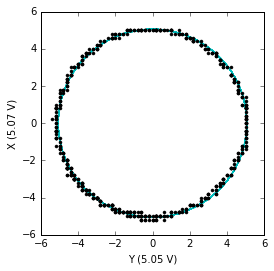
\includegraphics[scale=0.5]{1to1}
\caption{ Circle made by a frequency ratio of 1:1, with phase difference of $\frac{\pi}{2}$ radians.}
\label{fig:oscilloscope}
\end{figure}

\begin{figure}[h!]
\centering
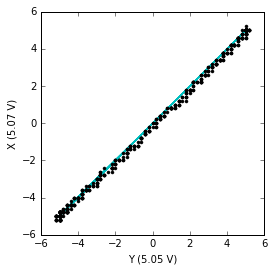
\includegraphics[scale=0.5]{1to1zero}
\caption{ Line made by a frequency ratio of 1:1, with phase difference of $0$ radians.}
\label{fig:oscilloscope}
\end{figure}

\begin{figure}[h!]
\centering
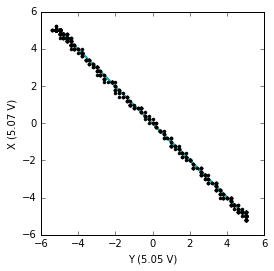
\includegraphics[scale=0.5]{1to1180}
\caption{ Line made by a frequency ratio of 1:1, with phase difference of $\pi$ radians.}
\label{fig:oscilloscope}
\end{figure}

\begin{figure}[h!]
\centering
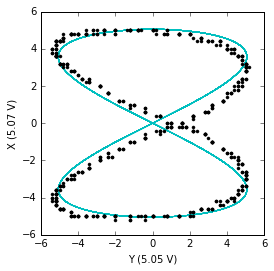
\includegraphics[scale=0.5]{1to1half}
\caption{ Figure made by a frequency ratio of 2:1.}
\label{fig:oscilloscope}
\end{figure}

\begin{figure}[h!]
\centering
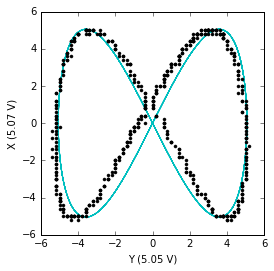
\includegraphics[scale=0.5]{1to2}
\caption{ Figure made by frequency ratio of 1:2.}
\label{fig:oscilloscope}
\end{figure}

\begin{figure}[h!]
\centering
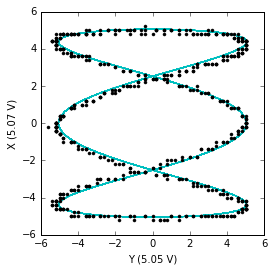
\includegraphics[scale=0.5]{1to1third}
\caption{ Figure created by a frequency ratio of 3:1.}
\label{fig:oscilloscope}
\end{figure}

\begin{figure}[h!]
\centering
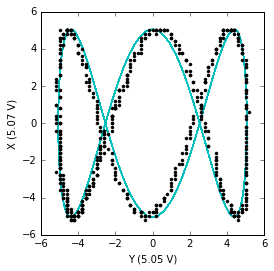
\includegraphics[scale=0.5]{1to3}
\caption{ Figure made by frequency ratio of 1:3.}
\label{fig:oscilloscope}
\end{figure}

\begin{figure}[h!]
\centering
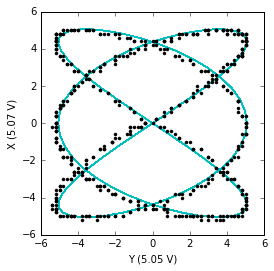
\includegraphics[scale=0.5]{1to2thirds}
\caption{ Figure made by frequency ratio of 3:2.}
\label{fig:oscilloscope}
\end{figure}

\begin{figure}[h!]
\centering
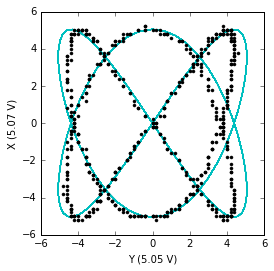
\includegraphics[scale=0.5]{1to3halves}
\caption{ Figure made by frequency ratio of 2:3.}
\label{fig:oscilloscope}
\end{figure}

\begin{figure}[h!]
\centering
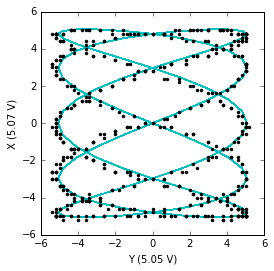
\includegraphics[scale=0.5]{1to2fifths}
\caption{ Figure made by frequency ratio of 5:2.}
\label{fig:oscilloscope}
\end{figure}

\begin{figure}[h!]
\centering
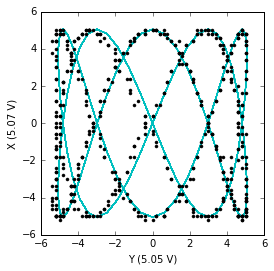
\includegraphics[scale=0.5]{1to5halves}
\caption{ Figure made by frequency ratio of 2:5.}
\label{fig:oscilloscope}
\end{figure}

\newpage

 \section*{Appendix B - Simulation of Lissajous curve }
 \label{sec:appendixB}
 \hspace{1cm}\\
Example: Figure 4 Simulation\\

import numpy as np

import matplotlib.pyplot as plt

import math as math\\

A1 = np.loadtxt('lissajous.txt',float)\\

t = A1[:,0]

y = A1[:,1]

x = A1[:,2]\\


Ax=5.05

Ay=5.07

wx = 1000

wy = 1000

phasex =0

phasey = math.pi/2\\


def XY(A,w,phase,t):

\hspace{1cm} return A*math.sin(2*math.pi*w*t + phase)\\

tpoints = np.arange(-0.020,0.02,0.00001)

xpoints = []

ypoints = []\\

for t in tpoints:

\hspace{1cm} xer = XY(Ax,wx,phasex,t)
    
\hspace{1cm} yer = XY(Ay,wy,phasey,t)
    
\hspace{1cm} xpoints.append(xer)
    
\hspace{1cm} ypoints.append(yer)\\
    
plt.plot(ypoints,xpoints,"c-")

plt.plot(y,x, "k.",label='IN')

plt.xlabel('Y (5.05 V)')

plt.ylabel('X (5.07 V)')

plt.show()

\end{document}